\documentclass[11pt]{article}

\usepackage[margin=0.9in]{geometry}
\usepackage{amsmath,amssymb}
\usepackage{booktabs}
\usepackage{enumitem}
\usepackage{listings}
\usepackage{xcolor}
\usepackage{hyperref}
\usepackage{graphicx}
\usepackage{float}      % optional, if you use [H]

\definecolor{backcolour}{rgb}{0.95,0.95,0.92}
\definecolor{codeblue}{rgb}{0.05,0.15,0.55}
\definecolor{codegreen}{rgb}{0.0,0.45,0.0}

\lstset{
    backgroundcolor=\color{backcolour},
    basicstyle=\ttfamily\small,
    keywordstyle=\color{codeblue}\bfseries,
    commentstyle=\color{codegreen},
    stringstyle=\color{purple},
    breaklines=true,
    frame=single,
    showstringspaces=false,
    tabsize=4
}

\title{CPSC 250 \\ Advanced Linear Regression Concepts}
\author{Edward Brash}
\date{}

\begin{document}

\maketitle

\section{Motivation}

In earlier lectures, we considered simple linear regression involving one independent variable.

Real-world data analysis is often more complicated.

In this lecture, we discuss:

\begin{itemize}
    \item multiple regression variables,
    \item parameter interpretation,
    \item correlations between variables,
    \item matrix representations,
    \item and data structures for regression.
\end{itemize}

\section{Complex Regression Problems}

Suppose we want to predict:

\[
y
\]

using several variables:

\[
x_1, x_2, x_3, x_4
\]

For example:

\begin{itemize}
    \item \(y\): housing price,
    \item \(x_1\): square footage,
    \item \(x_2\): zip code,
    \item \(x_3\): number of bedrooms,
    \item \(x_4\): number of bathrooms.
\end{itemize}

\section{The Regression Equation}

We seek an equation of the form:

\[
y =
\beta_0
+
\beta_1 x_1
+
\beta_2 x_2
+
\beta_3 x_3
+
\beta_4 x_4
\]

This is linear in the parameters.

\section{Why This Is Difficult}

Visualizing this problem directly would require a very high-dimensional plot.

For example:

\begin{itemize}
    \item one dependent variable,
    \item four independent variables.
\end{itemize}

This is impossible to visualize completely.

Therefore, regression becomes both:

\begin{itemize}
    \item a computational problem,
    \item and an interpretation problem.
\end{itemize}

\section{Parameter Uncertainties}

In practice, we determine:

\[
\beta_0 \pm \Delta\beta_0
\]

\[
\beta_1 \pm \Delta\beta_1
\]

and so on.

A parameter consistent with zero may indicate that the corresponding variable is not important.

For example:

\begin{quote}
If the coefficient for number of bedrooms is consistent with zero, housing prices may not strongly depend on that variable.
\end{quote}

\section{Exploratory Data Analysis}

Before fitting, we should first examine the data.

For example:

\[
y \text{ vs. } x_1
\]

\[
y \text{ vs. } x_2
\]

and so on.

This helps identify:

\begin{itemize}
    \item trends,
    \item bad data,
    \item outliers,
    \item nonlinear behavior.
\end{itemize}

\section{Correlations Between Variables}

Independent variables may themselves be correlated.

For example:

\[
x_2 \text{ vs. } x_3
\]

might show a strong trend.

This can produce misleading results.

\section{Correlation vs. Causation}

An important warning:

\begin{quote}
Correlation does not imply causation.
\end{quote}

Two variables may move together without one causing the other.

Regression analysis must therefore be interpreted carefully.

\section{Data Structures for Regression}

There are two common choices:

\begin{enumerate}
    \item NumPy arrays,
    \item pandas DataFrames.
\end{enumerate}

\section{Matrix Interpretation}

Suppose:

\[
y =
\beta_0
+
\beta_1 x_1
+
\beta_2 x_2
\]

for many data points.

We can write:

\[
y_1 =
\beta_0
+
\beta_1 x_{11}
+
\beta_2 x_{21}
\]

\[
y_2 =
\beta_0
+
\beta_1 x_{12}
+
\beta_2 x_{22}
\]

and so on.

\section{Matrix Form}

These equations can be rewritten as:

\[
\mathbf{y}
=
X
\mathbf{\beta}
\]

where:

\begin{itemize}
    \item \(\mathbf{y}\) is the vector of dependent values,
    \item \(X\) is the design matrix,
    \item \(\mathbf{\beta}\) is the parameter vector.
\end{itemize}

\begin{figure}[ht]
    \centering
    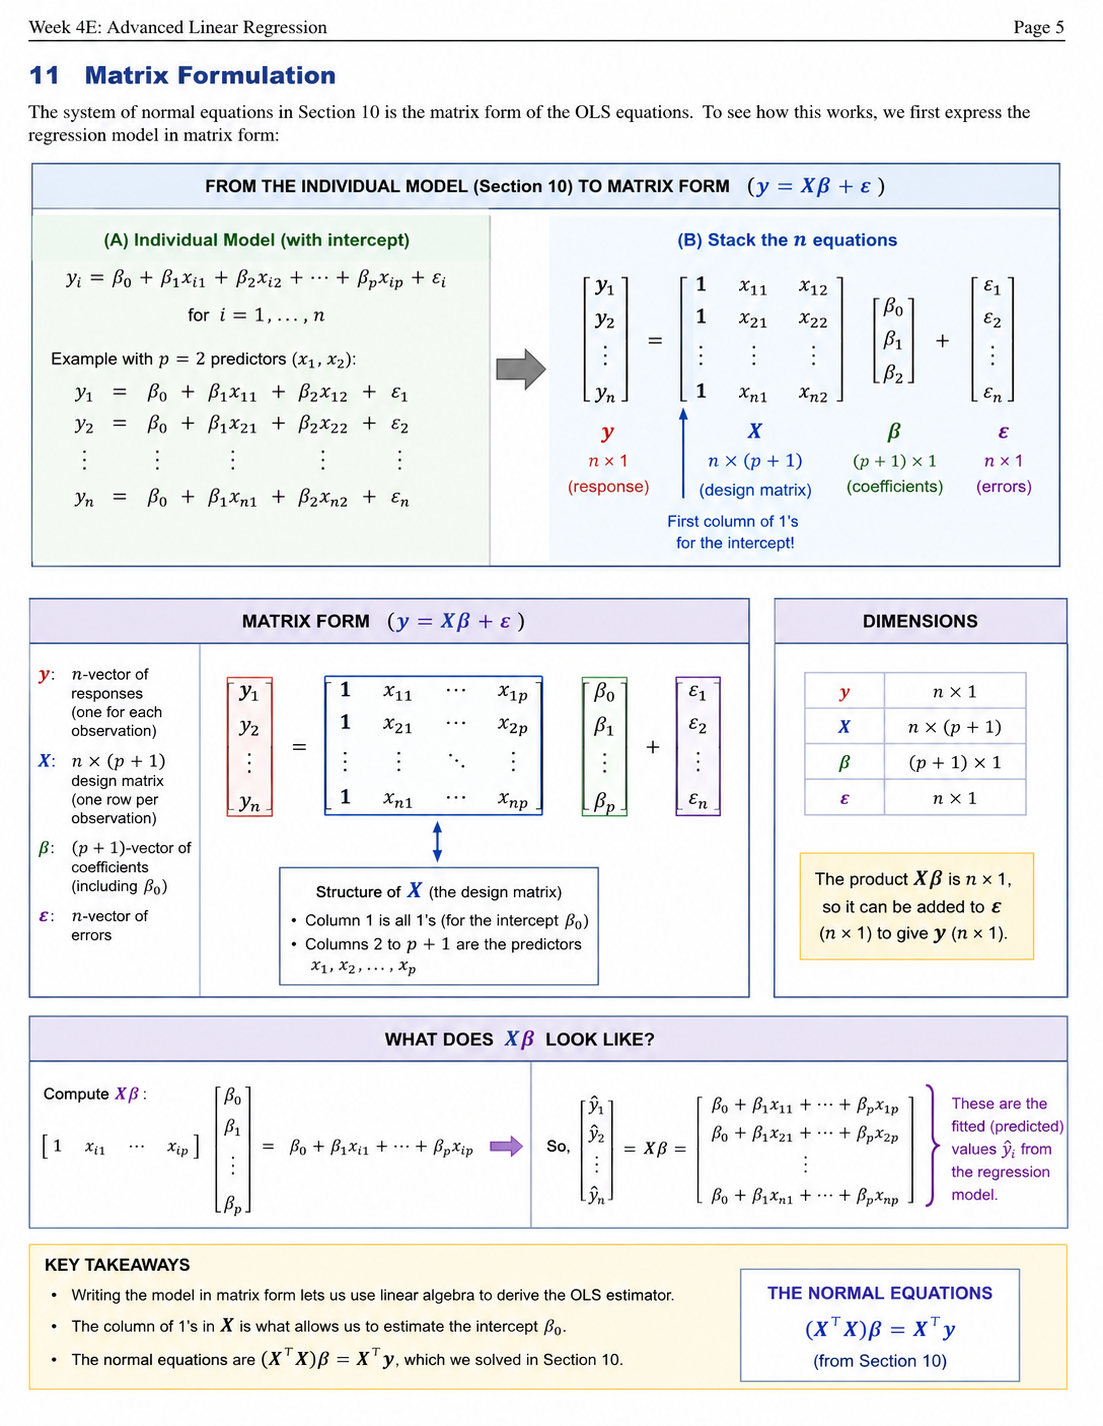
\includegraphics[width=\textwidth]{matrix_formulation_diagram.png}
    \caption{Moving from the individual regression equations to the matrix equation
    $\mathbf{y}=X\boldsymbol{\beta}+\boldsymbol{\epsilon}$. Notice that the first
    column of the design matrix $X$ consists entirely of ones. This column
    corresponds to the intercept coefficient $\beta_0$, which explains why
    packages such as \lstinline|statsmodels| require us to explicitly add a
    constant column using \lstinline|sm.add_constant(X)|.}
    \label{fig:matrix_formulation}
\end{figure}

\section{Solving for the Regression Parameters}

The matrix equation

\[
\mathbf{y}=X\boldsymbol{\beta}
\]

looks deceptively similar to an ordinary algebraic equation. Unfortunately, we
cannot simply "divide by $X$" because $X$ is generally \emph{not} a square
matrix.

Suppose there are $N$ data points and $M$ fitting parameters. Then

\[
X
\]

has dimensions

\[
N \times M.
\]

For example, if we fit a straight line,

\[
y=\beta_0+\beta_1x,
\]

to one hundred data points, then

\[
X
\]

has dimensions

\[
100 \times 2.
\]

Since $X$ is not square, the inverse

\[
X^{-1}
\]

does not exist.

The key idea is therefore to transform the problem into one involving a
\emph{square} matrix.

We do this by multiplying both sides of the equation by the transpose of $X$:

\[
X^T\mathbf{y}=X^TX\boldsymbol{\beta}.
\]

Now examine the dimensions:

\[
X^T
\quad\rightarrow\quad
M\times N
\]

and

\[
X
\quad\rightarrow\quad
N\times M.
\]

Therefore,

\[
X^TX
\]

has dimensions

\[
(M\times N)(N\times M)
=
M\times M.
\]

This is now a square matrix.

Provided the columns of $X$ are linearly independent, the matrix $X^TX$ is
invertible, allowing us to solve for the unknown parameter vector:

\[
\boxed{
\boldsymbol{\beta}
=
(X^TX)^{-1}X^T\mathbf{y}
}
\]

This equation is known as the \emph{normal equation} for linear least-squares
regression.

\subsection*{The Big Picture}

One of the most important ideas in this course is that we have transformed a
data-analysis problem into a linear algebra problem.

Originally, our goal was to determine the unknown regression parameters
$\beta_0,\beta_1,\ldots$ that best describe a set of measured data.

By constructing the design matrix $X$, we reformulated the problem as

\[
\mathbf{y}=X\boldsymbol{\beta},
\]

and ultimately reduced the entire regression problem to computing the inverse
of the matrix

\[
X^TX.
\]

Thus, from a computational point of view,

\[
\boxed{\text{Linear regression is fundamentally a matrix inversion problem.}}
\]

Modern software packages such as \lstinline|statsmodels| and
\lstinline|scikit-learn| hide these details from the user, but this is the
underlying mathematics that they are performing behind the scenes.

In principle:

\[
\mathbf{\beta}
=
(X^T X)^{-1} X^T \mathbf{y}
\]

This is the mathematical foundation of many regression algorithms.

\section{Important Practical Point}

For most Python regression tools:

\begin{itemize}
    \item \(X\)-data should be a two-dimensional matrix,
    \item \(y\)-data should be a one-dimensional array.
\end{itemize}

\section{Simple NumPy Example}

\begin{lstlisting}[language=Python]
import numpy as np

xi = [1, 2, 3, 4, 5]

yi = [1.1, 2.1, 2.9, 3.9, 5.1]

X = np.array(xi).reshape((-1,1))

y = np.array(yi)
\end{lstlisting}

\section{Why Reshape?}

The line:

\begin{lstlisting}[language=Python]
reshape((-1,1))
\end{lstlisting}

converts the array into a column matrix.

This is required because regression libraries expect:

\[
N \times M
\]

data structures for independent variables.

\section{Data Cleaning}

Before fitting, we should:

\begin{itemize}
    \item plot the data,
    \item look for missing points,
    \item identify outliers,
    \item think about appropriate models.
\end{itemize}

\section{Putting It All Together}

We now have all of the pieces needed to perform multiple linear regression on
a real dataset.

Suppose a company records the following information for many advertising
campaigns:

\begin{itemize}
    \item television advertising budget,
    \item radio advertising budget,
    \item newspaper advertising budget,
    \item resulting product sales.
\end{itemize}

Our goal is to determine how strongly each advertising medium influences sales.

Using the notation developed above, the regression model becomes

\[
\text{Sales}
=
\beta_0
+
\beta_1(\text{TV})
+
\beta_2(\text{Radio})
+
\beta_3(\text{Newspaper}).
\]

Each row of the design matrix corresponds to one advertising campaign, while
each column corresponds to one explanatory variable (plus the column of ones
used to determine the intercept).

Fortunately, Python libraries such as \lstinline|statsmodels| perform the
matrix computations automatically. The following example illustrates how this
is done in practice.

\section{Key Takeaways}

\begin{itemize}
    \item Real regression problems often involve many variables.
    \item Regression coefficients have uncertainties.
    \item Correlations between variables can complicate interpretation.
    \item Regression is fundamentally a linear-algebra problem.
    \item Most regression libraries require two-dimensional \(X\)-data.
    \item Exploratory plotting is extremely important before fitting.
\end{itemize}

\end{document}
